% ~3 pages. Numbers: README Sec. 3.3q (six environments; "CNN seeds 13 and 14" = the grey-box CNN numbers used here),
% 3.3r (Li readout, base). Figures and Table II: final/paper_figures.py -> figs/ (do not edit tab_envs.tex by hand).
% Every classifier number is against the two deployed classifiers (seeds 13, 14; generators trained on seed 11).
\section{Results}\label{sec:results}

\subsection{What Each Detector Sees}\label{sec:res-base}
Fig.~\ref{fig:base} shows damage and detection on one JSR axis at the ideal link.
Three groups of attackers separate by where their damage starts.
The generators and the pulsed jammer at low duty cycle break a tenth of the frames at $-22$ to $-19$\,dB, the genie flip, which must invert at least one symbol per frame, at $-15$\,dB, and barrage only at $-1.6$\,dB, 20\,dB later, because the matched filter rejects most of its power.
% pulsed p plateau: frames with no pulse at all = (1-p)^128 = 0.28 (p 0.01), 0.08 (p 0.02).
The pulsed jammer's damage saturates below one because at $p=0.01$ about $28\%$ of the frames receive no pulse at all.

The detectors order these attackers differently.
The classifier flags barrage on half of the frames at $-21$\,dB, 20\,dB before barrage does any damage, but the generators only at $-16$ to $-15$\,dB and the pulsed jammer at $-10$ to $-9$\,dB, when they already break $60$--$80\%$ of the frames.
Energy and kurtosis reach half of the frames for every in-band jammer at $-18$ to $-15$\,dB, and for barrage only at $-10$ and $-13$\,dB.
So the detector that is best against the jammer types it was trained on is the least sensitive against jammers matched to the victim's band.
At an excess FER of $0.1$, where we compare attackers below, energy flags the control and the generator trained against the classifier on $24$--$27\%$ of the frames, kurtosis on $7$--$11\%$ and the classifier on $11$--$17\%$, against a false-alarm rate of $5\%$.

\begin{figure*}[t]
\centering
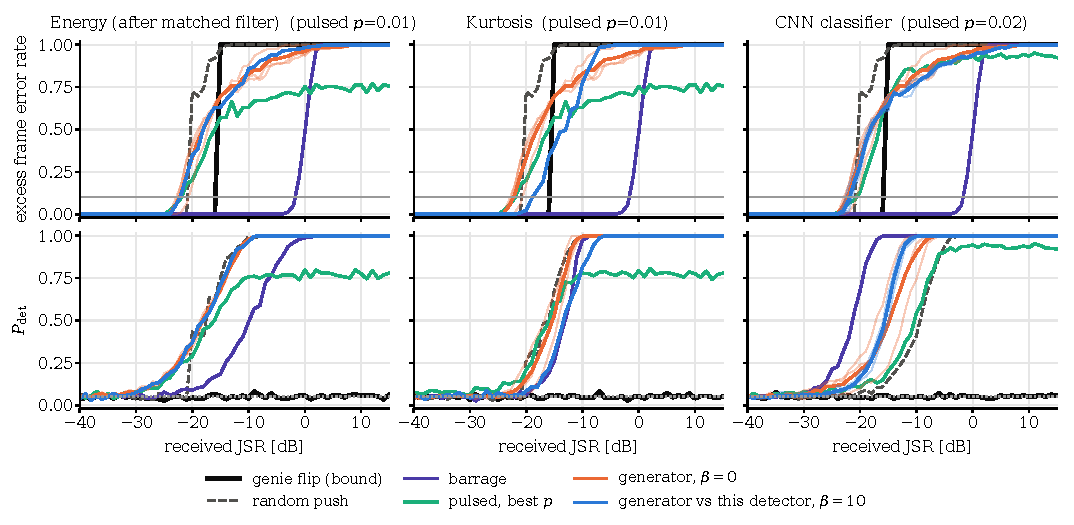
\includegraphics[width=\textwidth]{fig_base.pdf}
\caption{Damage (top) and per-frame detection probability (bottom) against the received JSR at the ideal link, $E_s/N_0=24$\,dB, one column per detector.
Generators: thick lines are the mean over three seeds, thin lines single seeds; the blue generator is trained against the column's detector.
The pulsed jammer is drawn at its best duty cycle $p$ for that detector.
Classifier column: mean over the two deployed classifiers, which the generators never saw.
Solid grey line: excess FER $0.1$; dotted: $\alpha=0.05$.}
\label{fig:base}
\end{figure*}

\subsection{Learned Versus Classical Jamming at Matched Damage}\label{sec:res-matched}
Table~\ref{tab:envs} and Fig.~\ref{fig:envs} give $P_{\mathrm{det}}$ at an excess FER of $0.1$ in all six environments.
% BER 3e-4: on/off reaches it jamming ~1 frame in 1500, so it sits at the FAR on every detector (README 3.3q).
At the lower level, an excess BER of $3\times10^{-4}$, the on/off jammer reaches the damage by jamming about one frame in $1500$ and stays at the false-alarm rate against every detector, so no attacker can do better there and we do not discuss that level further.

\emph{Against the classifier, the detector-aware generator gains at most 5 percentage points (pp) over the classical envelope.}
Its $P_{\mathrm{det}}$ differs from the envelope by $+0.4\pm1.3$, $-0.7\pm1.4$, $-4.7\pm0.5$, $+1.4\pm1.7$ and $+3.9\pm3.1$\,pp in the first five environments (mean $\pm$ standard error over generator seeds) and is $11$\,pp worse in \emph{both}, where two of its three seeds trained poorly and reach the matched damage only at $-12$ and $-11$\,dB instead of $-21$\,dB.
% README 3.3q Caveats: both, cnn_b10 r0/r2 damage onset -11/-12 dB; r1 0.054 ties the control.
Against the classifier the envelope is the pulsed jammer at $p=0.01$ or $0.02$ in every environment, at the edge of the family we ran.
Its one clear win, $-4.7$\,pp at \emph{noise\,1\,dB}, is not the detection term's: the control and the generators trained against energy and kurtosis are within $3$\,pp of the false-alarm rate there too (Sec.~\ref{sec:res-impair}).
There is little room to gain in any case: the genie flip, which no detector can see, is only $4$--$5$\,pp below the envelope.
The envelope also leaves the generator an advantage: the generator uses the victim's frame timing, which the pulsed jammer ignores.
Given the same timing, the pulsed jammer with one pulse in every frame is flagged by the classifier on $5$--$7\%$ of the frames, as often as the generator or less in every environment (within $1$\,pp at \emph{noise\,1\,dB}), and by energy and kurtosis about as often as the generator ($0.24$ and $0.12$ at the ideal link, against $0.24$ and $0.11$).
% numbers.json pulsed_sync_k1 vs cnn_b10. Classifier: 0.072/0.055/0.059/0.050/0.062/0.045 vs 0.113/0.086/0.051/0.100/0.135/0.203.

The one baseline the generators beat by a wide margin is the published generative jammer of Zhou et al.~\cite{11184988}, which is flagged on $98$--$100\%$ of the frames in every environment, $79$--$93$\,pp more than ours.
It is trained to imitate the victim's waveform, so it behaves as a matched-modulation jammer, and energy and kurtosis flag it too ($0.99$ and $0.98$ at the ideal link).

Against the other two detectors the picture does not favour learning either.
Against energy, on/off jamming beats every generator wherever energy works ($0.15$ against $0.22$--$0.38$).
Against kurtosis the control, which never saw a detector, is $3$--$7$\,pp below the envelope in every environment and $1$--$4$\,pp below the frame-timed pulsed jammer in five, the only detector where learning gains anything; the generator trained against kurtosis is no better than the control.

Training against the classifier itself buys nothing over training against a surrogate.
Against the classifier it trained on, the generator is flagged as often as against the two deployed ones, within $2$\,pp in five environments (Table~\ref{tab:envs}, white-box row).
The classifier's seed matters less still: across the three classifiers the envelope's standard deviation is at most $1.2$\,pp.
% README 3.3q "CNN seeds 13 and 14", findings 1-2.

\begin{table*}[t]
\caption{$P_{\mathrm{det}}$ at matched damage (excess FER $0.1$), $\alpha=0.05$. Mean $\pm$ standard deviation over generator seeds (three for the control and the generator trained against the classifier, one otherwise). Classifier block: mean over the two deployed classifiers.}
\label{tab:envs}
\centering\footnotesize
% generated by final/paper_figures.py -- do not edit by hand
\begin{tabular}{@{}lcccccc@{}}
\toprule
 & \emph{base} & \emph{noise} & \emph{noise\,1\,dB} & \emph{fading} & \emph{fading\,K28} & \emph{both} \\
\midrule
\multicolumn{7}{@{}l}{\emph{CNN classifier (deployed, grey-box)}} \\
\quad best classical & 0.11 & 0.09 & 0.10 & 0.09 & 0.10 & 0.09 \\
\quad pulsed, frame-timed ($k=1$) & 0.07 & 0.06 & 0.06 & 0.05 & 0.06 & 0.05 \\
\quad generator, $\beta=0$ & 0.17\,$\pm$\,0.10 & 0.05\,$\pm$\,0.01 & 0.05\,$\pm$\,0.00 & 0.06\,$\pm$\,0.01 & 0.08\,$\pm$\,0.01 & 0.05\,$\pm$\,0.01 \\
\quad generator vs CNN, $\beta=10$ & 0.11\,$\pm$\,0.02 & 0.09\,$\pm$\,0.03 & 0.05\,$\pm$\,0.01 & 0.10\,$\pm$\,0.03 & 0.14\,$\pm$\,0.05 & 0.20\,$\pm$\,0.12 \\
\quad Zhou et al.\ CGAN & 1.00 & 1.00 & 0.98 & 1.00 & 1.00 & 0.99 \\
\quad random push & 0.08 & 0.07 & 0.08 & 0.04 & 0.06 & 0.07 \\
\quad genie flip & 0.06 & 0.05 & 0.05 & 0.04 & 0.05 & 0.05 \\
\addlinespace[2pt]
\multicolumn{7}{@{}l}{\emph{CNN the generators trained against (white-box reference)}} \\
\quad generator vs CNN, $\beta=10$ & 0.11\,$\pm$\,0.02 & 0.10\,$\pm$\,0.04 & 0.05\,$\pm$\,0.02 & 0.10\,$\pm$\,0.01 & 0.13\,$\pm$\,0.05 & 0.13\,$\pm$\,0.07 \\
\addlinespace[2pt]
\multicolumn{7}{@{}l}{\emph{Energy (one-sided, after the matched filter)}} \\
\quad best classical & 0.15 & 0.15 & 0.15 & 0.04 & 0.05 & 0.04 \\
\quad pulsed, frame-timed ($k=1$) & 0.24 & 0.24 & 0.23 & 0.05 & 0.07 & 0.04 \\
\quad generator, $\beta=0$ & 0.27\,$\pm$\,0.04 & 0.26\,$\pm$\,0.02 & 0.24\,$\pm$\,0.02 & 0.05\,$\pm$\,0.01 & 0.06\,$\pm$\,0.01 & 0.05\,$\pm$\,0.01 \\
\quad generator vs energy, $\beta=10$ & 0.25 & 0.30 & 0.29 & 0.07 & 0.05 & 0.06 \\
\quad generator vs CNN, $\beta=10$ & 0.24\,$\pm$\,0.01 & 0.25\,$\pm$\,0.01 & 0.22\,$\pm$\,0.01 & 0.04\,$\pm$\,0.01 & 0.06\,$\pm$\,0.01 & 0.06\,$\pm$\,0.00 \\
\addlinespace[2pt]
\multicolumn{7}{@{}l}{\emph{Energy, channel gain known (fading environments)}} \\
\quad best classical & -- & -- & -- & 0.15 & 0.15 & 0.15 \\
\quad generator, $\beta=0$ & -- & -- & -- & 0.24\,$\pm$\,0.01 & 0.26\,$\pm$\,0.02 & 0.22\,$\pm$\,0.01 \\
\quad generator vs CNN, $\beta=10$ & -- & -- & -- & 0.25\,$\pm$\,0.04 & 0.24\,$\pm$\,0.00 & 0.45\,$\pm$\,0.18 \\
\addlinespace[2pt]
\multicolumn{7}{@{}l}{\emph{Kurtosis}} \\
\quad best classical & 0.14 & 0.13 & 0.13 & 0.14 & 0.14 & 0.13 \\
\quad pulsed, frame-timed ($k=1$) & 0.12 & 0.12 & 0.11 & 0.09 & 0.10 & 0.10 \\
\quad generator, $\beta=0$ & 0.07\,$\pm$\,0.01 & 0.09\,$\pm$\,0.01 & 0.09\,$\pm$\,0.01 & 0.10\,$\pm$\,0.01 & 0.08\,$\pm$\,0.02 & 0.09\,$\pm$\,0.01 \\
\quad generator vs kurtosis, $\beta=10$ & 0.11 & 0.08 & 0.11 & 0.07 & 0.10 & 0.08 \\
\quad generator vs CNN, $\beta=10$ & 0.11\,$\pm$\,0.01 & 0.09\,$\pm$\,0.04 & 0.10\,$\pm$\,0.01 & 0.11\,$\pm$\,0.00 & 0.07\,$\pm$\,0.01 & 0.38\,$\pm$\,0.25 \\
\bottomrule
\end{tabular}

\end{table*}

\begin{figure*}[t]
\centering
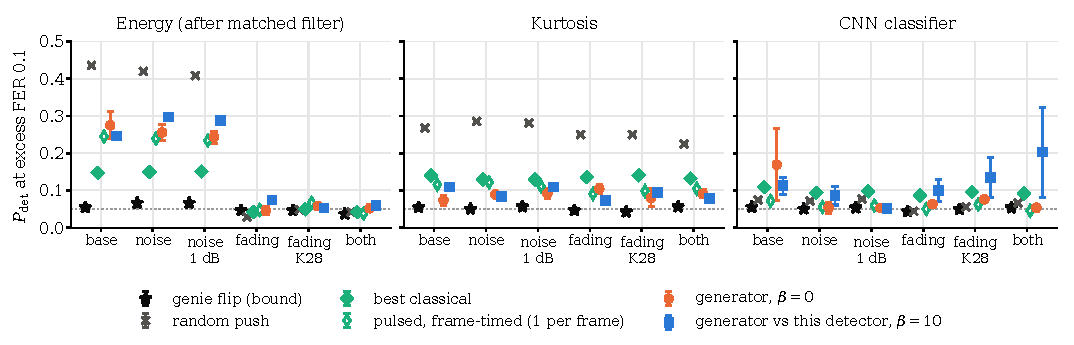
\includegraphics[width=\textwidth]{fig_envs.pdf}
\caption{$P_{\mathrm{det}}$ at matched damage (excess FER $0.1$) in the six environments; error bars are the standard deviation over generator seeds. Best classical: the classical envelope; frame-timed: the pulsed jammer with one pulse per frame. Zhou et al.'s generator ($0.98$--$1.00$ against the classifier) is off the scale. Dotted: $\alpha$.}
\label{fig:envs}
\end{figure*}

\subsection{Why the Detection Term Buys Nothing}\label{sec:res-why}
The control, trained for damage alone, is flagged by the classifier no more often than the detector-aware generator in five of six environments; at \emph{base} it is flagged $5.6\pm5.7$\,pp more often, driven by one seed at $0.28$.
Two observations explain why.

First, damage and stealth against the classifier point the same way.
At the ideal link the generator trained against the classifier puts $90\%$ of its in-band energy on about $1\%$ of the symbols, one burst per frame, an effective duty cycle of $0.010$--$0.012$, where the pulsed jammer is hardest for the classifier to detect ($p=0.01$--$0.02$).
% README 3.3r "What cnnGAN1 learned": p_eff = (E e_k)^2 / E e_k^2 at the decision points; calibrated Amuru p 0.01 -> 0.008.
Concentrating a fixed power budget on few symbols is what maximizes errors at a high signal-to-noise ratio~\cite{amuru2015optimal}, and such sparse bursts are what the classifier flags least (Sec.~\ref{sec:res-li}).
The generator thus rediscovers pulsed jamming, timed to the frame, which is why it ties with the pulsed jammer and does not beat its frame-timed variant.
% Measured for the CNN-targeted generator only (li/pulses.json); the control's duty cycle was not measured.

Second, the three detectors become sensitive at different powers, so penalizing all three cannot help.
Table~\ref{tab:transition} lists the JSR at which each detector flags white noise on half of the frames: at the ideal link the classifier transitions $7.7$\,dB below kurtosis and $10.9$\,dB below energy.
Where damage is cheap, around $-21$\,dB, only the classifier is active, and a generator trained against it is already at $0.24$ and $0.11$ on energy and kurtosis without a term for them.
We trained generators whose detection term is the largest of the three detectors' soft $P_{\mathrm{det}}$ per frame, with $\beta$ from $10$ to $100$, in shorter runs of $1500$ steps; the most-detecting detector flagged the best of them on $46\%$ of the frames at an excess FER of $0.1$, against $24\%$ for the generator trained against the classifier alone.
% README 3.3q "Does training against the whole detector suite help?": 1500-step white-box runs at base; worst-of-three
% 0.46 (CNN band) vs 0.24 (cnn_b10). Stealth ordering set by the transition spread, not by steps.

\begin{table}[t]
\caption{JSR [dB] at which white noise is flagged on half of the frames}
\label{tab:transition}
\centering\footnotesize
\begin{tabular}{@{}lcccccc@{}}
\toprule
 & \emph{base} & \emph{noise} & \emph{n.\,1\,dB} & \emph{fading} & \emph{f.\,K28} & \emph{both} \\
\midrule
Energy & $-10.0$ & $-10.1$ & $-10.0$ & $+7.1$ & $-1.1$ & $+6.8$ \\
Kurtosis & $-13.2$ & $-13.2$ & $-13.0$ & $-12.5$ & $-13.0$ & $-12.4$ \\
Classifier & $-20.9$ & $-18.4$ & $-16.0$ & $-20.9$ & $-21.2$ & $-17.8$ \\
\bottomrule
\end{tabular}
% artifacts/final/<env>/bands.json "transition" (classifier = the surrogate, seed 11).
\end{table}

\subsection{Impairments Split the Detectors}\label{sec:res-impair}
Each impairment disables a different detector and leaves the others in place (Table~\ref{tab:transition}, Fig.~\ref{fig:envs}).

Noise-level uncertainty costs the classifier sensitivity.
Its white-noise transition rises by $2.6$\,dB at $\sigma_N=0.5$\,dB and by $4.9$\,dB at $1$\,dB, and at $1$\,dB it flags the control and the generator trained against it at the false-alarm rate and the other generators on $7$--$8\%$ of the frames.
Energy after the matched filter is untouched: at $E_s/N_0=24$\,dB the noise is $0.4\%$ of the matched-filter energy, so a $1$\,dB error in it moves the clean statistic by about $0.1\%$, and the calibrated threshold rises from $1.29\%$ to $1.31\%$ above the clean mean.
% README 3.3q finding 4. The classifier's full-band spectrogram includes the out-of-band noise; that this is why it
% suffers is our reading, not tested.

Fading blinds the energy detector.
A Rician amplitude with $K=12$\,dB spreads the clean statistic so much that the threshold sits $61\%$ above the clean mean, the white-noise transition moves up by $17$\,dB, and no attacker is flagged on more than $14\%$ of the frames, the generators on $4$--$7\%$; at $K=28$\,dB the threshold is still $9.5\%$ above the mean.
Handed the true gain, the energy detector is unmoved: it flags the control on $22$--$26\%$ of the frames, as at the ideal link.
The classifier is unmoved by fading, and kurtosis, which is scale-free, by both impairments.
With both impairments, energy is blind, the classifier is weakened, and only kurtosis still flags the control above the false-alarm rate, on $9\%$ of the frames.
% both: control energy 0.052, CNN 0.054 (deployed), kurtosis 0.091; envelope kurtosis 0.132.

\subsection{Scored the Way Li et al.\ Score It}\label{sec:res-li}
Li et al.~\cite{li2022jamming_ofdm} score their classifier per image by its arg-max decision on their own jammer types, over a JSR range of $-20$ to $+10$\,dB.
Scored that way at the ideal link, our retrained classifier detects their four types with $92.6\%$ accuracy at a clean false-alarm rate of $0.8\%$; they report $100\%$, and we attribute the gap to the bottom of that range, which lies below our receiver noise.
Table~\ref{tab:li} reads the same arg-max decision at matched damage, against a generator trained against a surrogate classifier.
At half the frames lost, the classifier flags the generator on $9\%$ of the frames and the pulsed jammer at $p=0.02$ on $5\%$, against $52\%$ for Li et al.'s protocol-aware type and $100\%$ for their other three.
At a complete loss of the link, the generator is flagged on every frame, while the pulsed jammer at $p=0.05$ still escapes on $82\%$.
A classifier scored on the types it was trained on thus overstates what it detects; at matched damage the pulsed jammers, not the learned one, expose the gap.

\begin{table}[t]
\caption{Classifier arg-max detection rate at matched damage, ideal link (Li et al.'s scoring; clean false-alarm rate $0.8\%$)}
\label{tab:li}
\centering\footnotesize
\begin{tabular}{@{}lccc@{}}
\toprule
Excess FER & $0.1$ & $0.5$ & $0.9$ \\
\midrule
Generator vs a surrogate classifier & $0.03$ & $0.09$ & $1.00$ \\
Pulsed, $p=0.02$ & $0.04$ & $0.05$ & $0.68$ \\
Pulsed, $p=0.05$ & $0.04$ & $0.08$ & $0.18$ \\
Protocol-aware~\cite{li2022jamming_ofdm} ($p=0.25$) & $0.37$ & $0.52$ & $0.67$ \\
Barrage, tone, pulse comb~\cite{li2022jamming_ofdm} & $1.00$ & $1.00$ & $1.00$ \\
Genie flip & $0.01$ & $0.01$ & $0.01$ \\
\bottomrule
\end{tabular}
% README 3.3r: deployed = seed 11, surrogate = seed 12 (cnn_b10_grey, 3 seeds); argmax; Li window -20..+10 dB.
\end{table}
